\documentclass{standalone}
\usepackage{tikz}
\usetikzlibrary{patterns, positioning}


\begin{document}
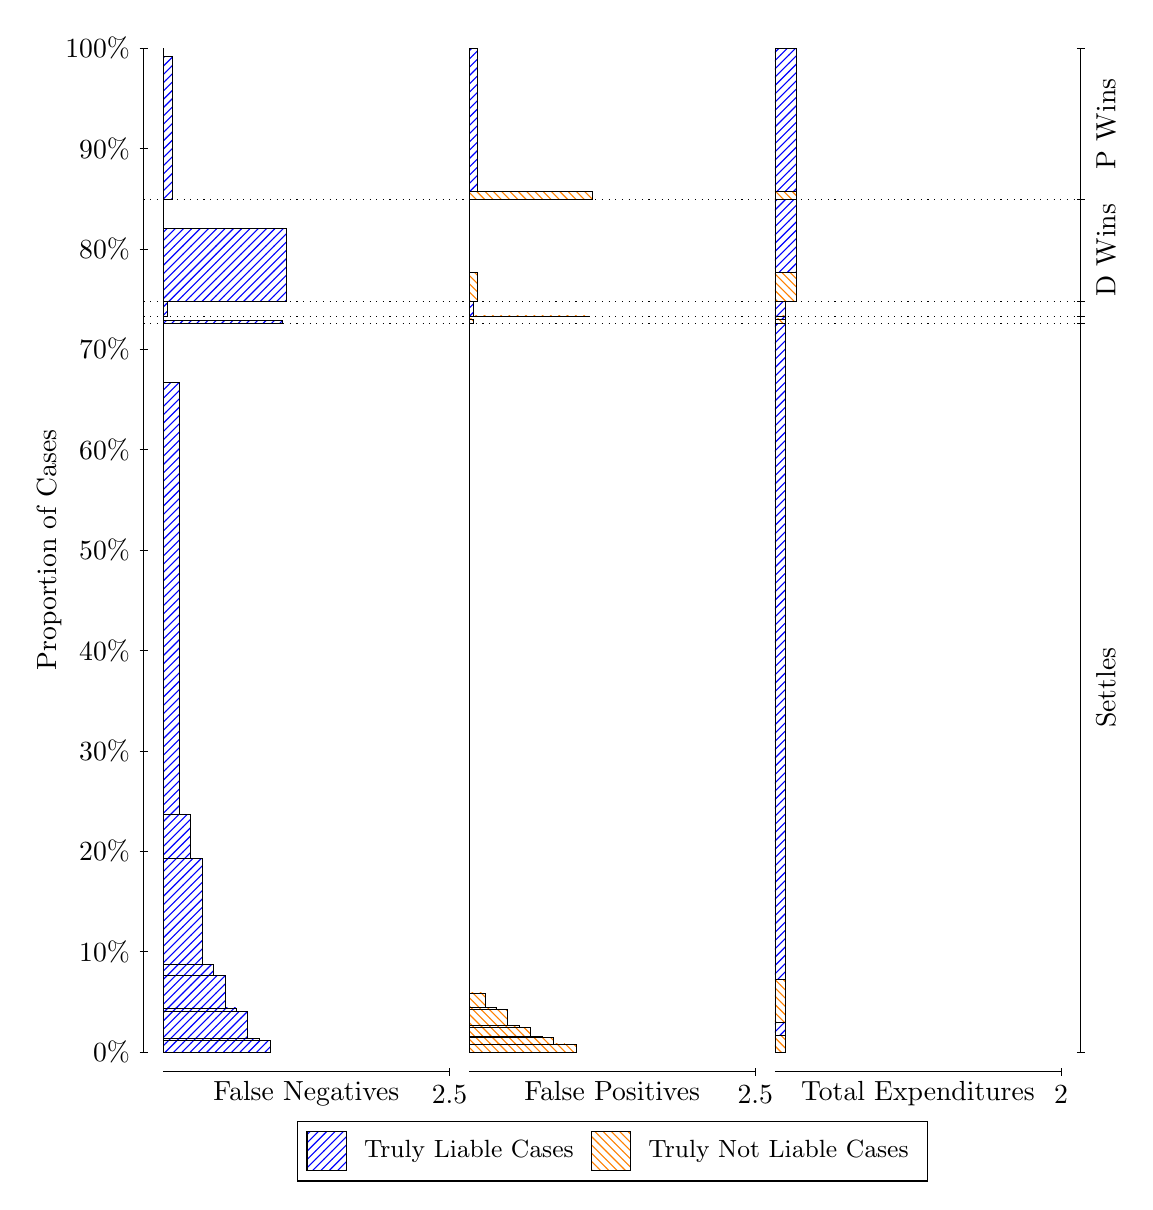
\begin{tikzpicture}
\draw[black, very thin] (1.5,1.75) -- (1.5,14.5);
\node[rotate=90, text=black, anchor=center] at (0.3, 8.125) {Proportion of Cases};
\draw[black, very thin] (1.45,1.75) -- (1.55,1.75);
\node[text=black, anchor=east] at (1.45, 1.75) {0\%};
\draw[black, very thin] (1.45,3.025) -- (1.55,3.025);
\node[text=black, anchor=east] at (1.45, 3.025) {10\%};
\draw[black, very thin] (1.45,4.3) -- (1.55,4.3);
\node[text=black, anchor=east] at (1.45, 4.3) {20\%};
\draw[black, very thin] (1.45,5.575) -- (1.55,5.575);
\node[text=black, anchor=east] at (1.45, 5.575) {30\%};
\draw[black, very thin] (1.45,6.85) -- (1.55,6.85);
\node[text=black, anchor=east] at (1.45, 6.85) {40\%};
\draw[black, very thin] (1.45,8.125) -- (1.55,8.125);
\node[text=black, anchor=east] at (1.45, 8.125) {50\%};
\draw[black, very thin] (1.45,9.4) -- (1.55,9.4);
\node[text=black, anchor=east] at (1.45, 9.4) {60\%};
\draw[black, very thin] (1.45,10.675) -- (1.55,10.675);
\node[text=black, anchor=east] at (1.45, 10.675) {70\%};
\draw[black, very thin] (1.45,11.95) -- (1.55,11.95);
\node[text=black, anchor=east] at (1.45, 11.95) {80\%};
\draw[black, very thin] (1.45,13.225) -- (1.55,13.225);
\node[text=black, anchor=east] at (1.45, 13.225) {90\%};
\draw[black, very thin] (1.45,14.5) -- (1.55,14.5);
\node[text=black, anchor=east] at (1.45, 14.5) {100\%};

\draw[black, very thin] (13.4,1.75) -- (13.4,14.5);
\draw[black, very thin] (13.35,1.75) -- (13.45,1.75);
\node[anchor=west] at (13.35, 1.75) {};
\draw[black, very thin] (13.35,11.004) -- (13.45,11.004);
\node[anchor=west] at (13.35, 11.004) {};
\draw[black, very thin] (13.35,11.095) -- (13.45,11.095);
\node[anchor=west] at (13.35, 11.095) {};
\draw[black, very thin] (13.35,11.285) -- (13.45,11.285);
\node[anchor=west] at (13.35, 11.285) {};
\draw[black, very thin] (13.35,12.575) -- (13.45,12.575);
\node[anchor=west] at (13.35, 12.575) {};
\draw[black, very thin] (13.35,14.5) -- (13.45,14.5);
\node[anchor=west] at (13.35, 14.5) {};

\draw[black, very thin, pattern color=blue, pattern=north east lines] (1.75,1.75) rectangle (3.1125,1.8988);
\draw[black, very thin, pattern color=blue, pattern=north east lines] (1.75,1.8988) rectangle (2.9672,1.9201);
\draw[black, very thin, pattern color=blue, pattern=north east lines] (1.75,1.9201) rectangle (2.8218,2.2643);
\draw[black, very thin, pattern color=blue, pattern=north east lines] (1.75,2.2643) rectangle (2.6765,2.3112);
\draw[black, very thin, pattern color=blue, pattern=north east lines] (1.75,2.3112) rectangle (2.5312,2.7261);
\draw[black, very thin, pattern color=blue, pattern=north east lines] (1.75,2.7261) rectangle (2.3858,2.8657);
\draw[black, very thin, pattern color=blue, pattern=north east lines] (1.75,2.8657) rectangle (2.2405,4.2109);
\draw[black, very thin, pattern color=blue, pattern=north east lines] (1.75,4.2109) rectangle (2.0952,4.7667);
\draw[black, very thin, pattern color=blue, pattern=north east lines] (1.75,4.7667) rectangle (1.9498,10.253);
\draw[black, very thin, pattern color=orange, pattern=north west lines] (1.75,10.253) rectangle (1.75,11.004);
\draw[black, very thin, pattern color=blue, pattern=north east lines] (1.75,11.004) rectangle (3.2578,11.039);
\draw[black, very thin, pattern color=orange, pattern=north west lines] (1.75,11.039) rectangle (1.75,11.095);
\draw[black, very thin, pattern color=blue, pattern=north east lines] (1.75,11.095) rectangle (1.8045,11.283);
\draw[black, very thin, pattern color=orange, pattern=north west lines] (1.75,11.283) rectangle (1.75,11.285);
\draw[black, very thin, pattern color=blue, pattern=north east lines] (1.75,11.285) rectangle (3.3123,12.213);
\draw[black, very thin, pattern color=orange, pattern=north west lines] (1.75,12.213) rectangle (1.75,12.575);
\draw[black, very thin, pattern color=blue, pattern=north east lines] (1.75,12.575) rectangle (1.859,14.398);
\draw[black, very thin, pattern color=orange, pattern=north west lines] (1.75,14.398) rectangle (1.75,14.5);
\draw[black, very thin, pattern color=orange, pattern=north west lines] (5.6333,1.75) rectangle (6.9958,1.8424);
\draw[black, very thin, pattern color=orange, pattern=north west lines] (5.6333,1.8424) rectangle (6.8505,1.8514);
\draw[black, very thin, pattern color=orange, pattern=north west lines] (5.6333,1.8514) rectangle (6.7052,1.935);
\draw[black, very thin, pattern color=orange, pattern=north west lines] (5.6333,1.935) rectangle (6.5598,1.9495);
\draw[black, very thin, pattern color=orange, pattern=north west lines] (5.6333,1.9495) rectangle (6.4145,2.066);
\draw[black, very thin, pattern color=orange, pattern=north west lines] (5.6333,2.066) rectangle (6.2692,2.0866);
\draw[black, very thin, pattern color=orange, pattern=north west lines] (5.6333,2.0866) rectangle (6.1238,2.2928);
\draw[black, very thin, pattern color=orange, pattern=north west lines] (5.6333,2.2928) rectangle (5.9785,2.3147);
\draw[black, very thin, pattern color=orange, pattern=north west lines] (5.6333,2.3147) rectangle (5.8332,2.5017);
\draw[black, very thin, pattern color=blue, pattern=north east lines] (5.6333,2.5017) rectangle (5.6333,11.004);
\draw[black, very thin, pattern color=orange, pattern=north west lines] (5.6333,11.004) rectangle (5.6878,11.061);
\draw[black, very thin, pattern color=blue, pattern=north east lines] (5.6333,11.061) rectangle (5.6333,11.095);
\draw[black, very thin, pattern color=orange, pattern=north west lines] (5.6333,11.095) rectangle (7.1412,11.098);
\draw[black, very thin, pattern color=blue, pattern=north east lines] (5.6333,11.098) rectangle (5.6878,11.285);
\draw[black, very thin, pattern color=orange, pattern=north west lines] (5.6333,11.285) rectangle (5.7423,11.647);
\draw[black, very thin, pattern color=blue, pattern=north east lines] (5.6333,11.647) rectangle (5.6333,12.575);
\draw[black, very thin, pattern color=orange, pattern=north west lines] (5.6333,12.575) rectangle (7.1957,12.677);
\draw[black, very thin, pattern color=blue, pattern=north east lines] (5.6333,12.677) rectangle (5.7423,14.5);
\draw[black, very thin, pattern color=orange, pattern=north west lines] (9.5167,1.75) rectangle (9.6529,1.9589);
\draw[black, very thin, pattern color=blue, pattern=north east lines] (9.5167,1.9589) rectangle (9.6529,2.1291);
\draw[black, very thin, pattern color=orange, pattern=north west lines] (9.5167,2.1291) rectangle (9.6529,2.6719);
\draw[black, very thin, pattern color=blue, pattern=north east lines] (9.5167,2.6719) rectangle (9.6529,11.004);
\draw[black, very thin, pattern color=orange, pattern=north west lines] (9.5167,11.004) rectangle (9.6529,11.061);
\draw[black, very thin, pattern color=blue, pattern=north east lines] (9.5167,11.061) rectangle (9.6529,11.095);
\draw[black, very thin, pattern color=orange, pattern=north west lines] (9.5167,11.095) rectangle (9.6529,11.098);
\draw[black, very thin, pattern color=blue, pattern=north east lines] (9.5167,11.098) rectangle (9.6529,11.285);
\draw[black, very thin, pattern color=orange, pattern=north west lines] (9.5167,11.285) rectangle (9.7892,11.647);
\draw[black, very thin, pattern color=blue, pattern=north east lines] (9.5167,11.647) rectangle (9.7892,12.575);
\draw[black, very thin, pattern color=orange, pattern=north west lines] (9.5167,12.575) rectangle (9.7892,12.677);
\draw[black, very thin, pattern color=blue, pattern=north east lines] (9.5167,12.677) rectangle (9.7892,14.5);
\draw[black, dotted] (1.5,11.004) -- (13.4,11.004);
\draw[black, dotted] (1.5,11.095) -- (13.4,11.095);
\draw[black, dotted] (1.5,11.285) -- (13.4,11.285);
\draw[black, dotted] (1.5,12.575) -- (13.4,12.575);
\draw[black, very thin] (1.75,1.5) -- (5.3833,1.5);
\node[text=black, anchor=north] at (3.5667, 1.5) {False Negatives};
\draw[black, very thin] (5.3833,1.45) -- (5.3833,1.55);
\node[text=black, anchor=north] at (5.3833, 1.45) {2.5};

\draw[black, very thin] (5.6333,1.5) -- (9.2667,1.5);
\node[text=black, anchor=north] at (7.45, 1.5) {False Positives};
\draw[black, very thin] (9.2667,1.45) -- (9.2667,1.55);
\node[text=black, anchor=north] at (9.2667, 1.45) {2.5};

\draw[black, very thin] (9.5167,1.5) -- (13.15,1.5);
\node[text=black, anchor=north] at (11.333, 1.5) {Total Expenditures};
\draw[black, very thin] (13.15,1.45) -- (13.15,1.55);
\node[text=black, anchor=north] at (13.15, 1.45) {2};

\node[text=black, centered, rotate=90] at (13.72, 6.3772) {Settles};


\node[text=black, centered, rotate=90] at (13.72, 11.93) {D Wins};
\node[text=black, centered, rotate=90] at (13.72, 13.537) {P Wins};

\draw (7.449999999999999,1.5) node[draw=none] (baseCoordinate) {};
\begin{scope}[align=center]
        \matrix[scale=0.5, draw=black, below=0.5cm of baseCoordinate, nodes={draw}, column sep=0.1cm]{
            \node[rectangle, draw, minimum width=0.5cm, minimum height=0.5cm, pattern color=blue, pattern=north east lines] {}; &
            \node[draw=none, font=\small, text=black] (B) {Truly Liable Cases}; &
            \node[rectangle, draw, minimum width=0.5cm, minimum height=0.5cm, pattern color=orange, pattern=north west lines] {}; &
            \node[draw=none, font=\small, text=black] (B) {Truly Not Liable Cases}; \\
            };
\end{scope}

\end{tikzpicture}
\end{document}